\chapter{Results}
\label{chap:res}
In this section we will present and discuss the results from the experiments on the REST implementation. The experiments were conducted on an Intel(R) Xeon(R) Gold 6426Y processor with 500 GB RAM. Samples from the Porto dataset are used as data.

For these experiments there are many parameters that can be adjusted. To keep this section concise we will only analyze the parameters that are most relevant to our research questions. Other parameters are set using the experimental results from \textcite{zhao2018rest}. For example, the spatial deviation threshold for an MRT, definition \ref{def:mrt}, is set to $\epsilon_s = 200 m$, because it produced the best results in the previous experiments. The \textit{Compression Threshold} for the reference set construction as shown in code listing \ref{lst:ca_og} is set to $CT = 3$. In the experiments from \textcite{zhao2018rest}, both $CT =3$ and $CT = 5$ were tested. The latter showed slightly better results, but in our experience, it was slower. Therefore, we set $CT = 3$ despite slightly worse performance, due to time constraints. Additionally, as long as all variants use the same parameter, the comparisons will be valid and likely hold true for both thresholds.

To describe different variants of REST, labels for each variant have been created. The spatial filter variant is denoted by the suffix \textit{-SFX}, where \textit{X} is the window size in meters. The Sakoe-Chiba band is denoted by the suffix \textit{-BNDX}, where \textit{X} is the band size. The KNN variant is denoted by the suffix \textit{-KNNX}, where \textit{X} is the number of MRTs selected. An example label can be \textit{REST-SF75-KNN3-BND20}, which represents REST using a spatial filter with window size of $75\times75 m^2$, selecting the 3 best MRTs, and applying a Sakoe-Chiba band of size 20 to each Max DTW calculation.

\section{Compression Ratio and Runtime}
In order to answer RQ1 REST and the variants have been measured when compressing trajectories. These experiments have been executed by first building a reference set with a sample size of 10K, to then use the reference set during compression. The trajectories in the sample used to build the reference set were excluded from the later compression, since they would have a much higher compression ratio than other trajectories. Additionally, in order to answer RQ2, DP-DTW has been measured when compressing the same amount of trajectories, using the same spatial deviation threshold. However, DP-DTW was incredibly slow and there was only time to run the tests to compress 5K trajectories. This run took 20 hours and the average compression ratio was 1.7. Note that the average and total compression ratio is the same for DP-DTW since there is no reference set.

\begin{figure}[h]
    \begin{minipage}{0.99\linewidth}
        \centering
        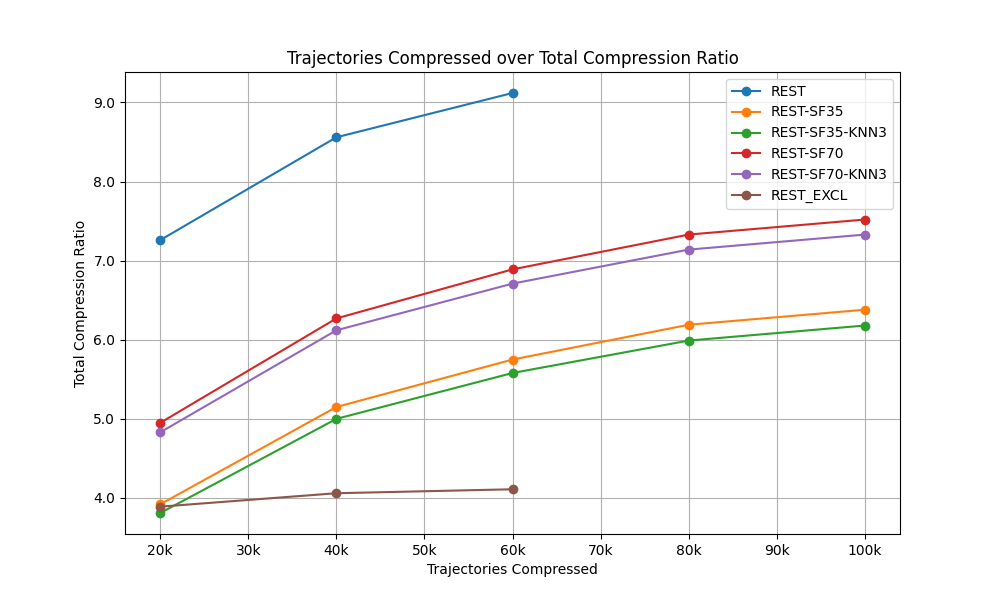
\includegraphics[height=7cm, keepaspectratio]{../code/plotting/tot_compression.png}
        \caption{Total Compression Ratio over trajectories compressed. The reference set was constructed using a sample size of 10K.}
        \label{fig:n_compression}
    \end{minipage}
\end{figure}

In figure \ref{fig:n_compression} it is clear that REST has the best compression ratio. It has a total compression ratio of $5.55$ for 60K compressed trajectories. Note that REST and XREST only compressed 60K trajectories instead of 100K due to time constraints, in both figure \ref{fig:n_compression} and figure \ref{fig:n_runtime}. The spatial filter variants have a lower compression ratio than REST, but it increases with a larger window size. This outcome is expected because REST can be seen as having an infinitely large window size. Therefore, when it comes to RQ1, this shows that the spatial filter variant with a sufficiently large window size can reach close to the same compression ratio as REST. The KNN variants in combination with the spatial filter shows promising results as they only slightly reduce the compression ratio compared to spatial filter with no KNN. For instance, \textit{REST-SF120-KNN3} has a total compression ratio of $4.86$ for 60K compressed trajectories, the corresponding number for \textit{REST} is $5.55$. This shows that \textit{REST-SF120-KNN3} achieves 87\% of \textit{REST}'s compression ratio.

KNN used directly on REST did not show promising results and is therefore not shown in the results. This is likely because REST uses all reference trajectories to search for MRTs, whereas selecting a handful early in the process seems to miss out on better suggestions.

In general the total compression grows as more trajectories are compressed. This is because the number of compressed trajectories grows larger in relation to the set size. From equation \ref{eq:tot_cr}, this represents \textit{points\_in\_set} becoming smaller compared to \textit{all\_points}. In the case where the amount of compressed trajectories keeps growing, the size of the reference set would eventually become negligible, causing the total compression to approach the average compression. The average compression ratio (not shown), stays near the same level for all variants, around $7.4$ for REST. Moreover, the amount of compressions needed to make the reference set negligible is much greater than any realistic use case. The result in our experiments is that the total compression grows slower and slower.

XREST has a much lower compression ratio than REST and REST-based variants. This indicates that the reference set of XREST has low coverage. This is somewhat expected as the exclusive strategy of XREST requires a larger sample size to achieve the same coverage as REST. Additionally, this can be due to differences in the length of the reference trajectories. Shorter reference trajectories lead to a longer and less efficient compression sequences. Another difference between REST and XREST is the slower growth of the compression ratio for XREST. This is because XREST has a smaller reference set, thereby noticing less of a change as the number of trajectories compressed increase.

DP-DTW has a compression ratio of 1.7 for 5K trajectories. The compression ratio will not change as more trajectories are compressed, since DP-DTW is a local strategy only looking at one trajectory at a time. Therefore, we can use the results for 5K when comparing to REST based variants for 100K compressed trajectories.

DP-DTW's compression ratio is estimated to be more than 3 times lower than REST's. This suggests that a line simplification algorithm can not achieve the same compression ratio as a reference-based strategy. In regard to RQ2 this is a strong indication that the reference-based strategy is superior to DP-DTW in terms of compression ratio. DP-DTW only considers one trajectory at a time and does not benefit from any similarities between trajectories in the dataset as a whole. REST uses the similarities for a much more effective compression. Additionally, in the experiments of \textit{zhao2018rest}, they compared DP with SED as the accuracy metric to REST, and these results also showed a much lower compression ratio using line simplification.

\begin{figure}[h]
    \begin{minipage}{0.99\linewidth}
        \centering
        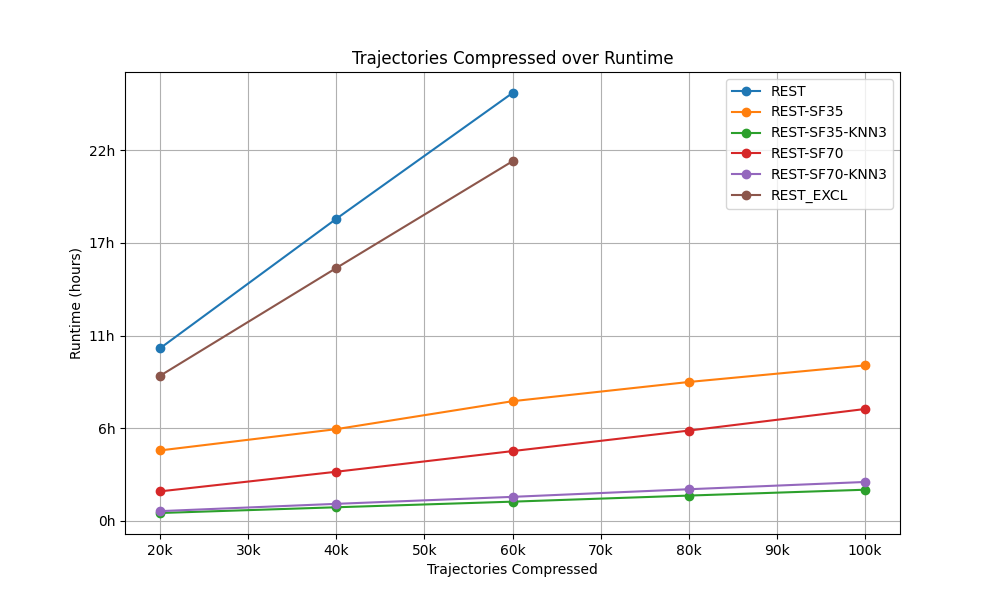
\includegraphics[height=7cm, keepaspectratio]{../code/plotting/n_runtime.png}
        \caption{Runtime over trajectories compressed. The reference set construction is included in the time, using a 10K sample size.}
        \label{fig:n_runtime}
    \end{minipage}
\end{figure}

In figure \ref{fig:n_runtime} we see that REST and XREST are significantly slower than other variants. This demonstrates the inefficiency of using the entire reference set as candidates in MRT search. XREST is slightly faster than REST, this is because the reference set is smaller, leading to fewer reference trajectories to search through. Although, with a smaller reference set we would expect XREST to be even faster. This indicates that the quality of the reference set is slowing it. XREST has shorter trajectories in the reference set, causing a more segmented compression sequence.

The spatial filter variants are significantly faster than REST and XREST. The spatial filter efficiently selects a subset of the reference set to use for MRT search. Note that \textit{REST-SF70} has approximately the same runtime \textit{REST-SF120}, this is unexpected as a smaller window size is expected to find candidate reference trajectories, and hence do fewer trajectory comparisons. Nonetheless, the smaller window size is equally fast. Presumably, this is because the reference set is bigger. When using a smaller window size, fewer trajectories are found in reference set construction as well, leading to a larger set. With a larger set, there are more trajectory comparisons even within the smaller window size, leading to a slower runtime.

We see that the KNN variants in combination with a spatial filter lead to a faster runtime. Interestingly, Also note that \textit{XREST-SF120} is 35 times slower than \textit{XREST-SF120-KNN3}. This shows that KNN had a good impact when using XREST with a spatial filter to reduce runtime. It also had a good impact for REST, but not as large as with XREST. \textit{REST-SF120-KNN3} compresses the same amount of trajectories 9 times faster than \textit{REST}. Considering RQ2, this shows a significant speed-up of the original REST algorithm.

DP-DTW is the slowest of all the compression algorithms. Based on the measurements it is estimated to be 8 times slower than \textit{REST} and 126 times slower than \textit{REST-SF120-KNN3}. This is because it performs many DTW comparisons which are expensive. DP-DTW calculates the Max DTW distance between the simplified trajectory and the complete trajectory for each iteration. The complete trajectory has the full length of the original trajectory, while the simplified trajectory begins with length two and grows from there. Because DTW is $O(N \times M)$, where $N$ and $M$ are the lengths of the trajectories, and $N$ is always the full trajectory length, this will be an expensive process. In terms of RQ2, we see that REST significantly outperforms DP-DTW in terms of runtime and the REST variation using a spatial filter with KNN drastically outperforms it. In reflection, this DP implementation is too simple, it compresses 250 trajectories per hour on average. It cannot be considered to be a fair representation of non reference-based methods. To fully answer RQ2 more non reference-based methods must be compared with REST.

All in all, when looking at both compression ratio and runtime, we can see that the spatial filter variants are much faster than REST and XREST, while still achieving high compression ratios. In regard to RQ1, the best performing variant \textit{REST-SF120-KNN3}, achieved 87\% of \textit{REST}'s compression ratio, but 9 times faster. In terms of achieving similar compression ratios, this is clearly the case for this variant. Although the increase in runtime can be considered significant, it also reflects some limitations for using REST. All REST variants are limited by the speed of the Max DTW calculation, this is the bottleneck for runtime. Speed-ups larger than what is achieved by \textit{REST-SF120-KNN3}, will likely require a cheaper trajectory comparison. Nevertheless, the benefit of using DTW is that it provides a high quality similarity comparison.

Considering that Max DTW is the most resource demanding part of the algorithm, it would be interesting to test REST using another trajectory distance measure. The variants created in this thesis will likely improve the performance for REST with another trajectory comparison as well, because it is the main operation.

The DP implementation used as a comparison in the experiments conducted by \textcite{zhao2018rest} in their study, was SED based. This implementation was much faster than the different REST strategies. Therefore, it would be interesting to see how REST would perform using a "Max SED" distance instead of a Max DTW distance for the MRTs spatial deviation threshold. This change would likely result in a faster runtime.

However, it is important to note that in this case, the quality of compression would not be the same, because SED and Max DTW are different metrics. Hence, a direct comparison between them would not be meaningful. Nonetheless, it would be interesting to compare a SED based REST and a Max DTW based REST through a practical application. For instance through querying the compressed trajectories and comparing the quality of the result, in relation to the achieved compression ratio and runtime efficiency.

\textit{REST} is slow, but achieves a high compression ratio by using the entire reference set for each compression. XREST has the lowest compression ratio and the second-highest runtime, however, using a spatial filter and KNN it, is significantly faster than all other variants. This shows that the strategy is unable to compete with REST in terms of compression ratio, but has the best runtime. The low compression ratio might be due to the sample size being too small, or shorter reference trajectories in the reference set.

A version of XREST with an improved compression ratio could compete with REST in both runtime and compression ratio. The strategy seems to speed up significantly when using a spatial filter with KNN, while keeping a similar compression ratio. Nonetheless, the compression ratio is low, and there can be multiple reasons for this. Among them are different qualities of the reference set, too low sample size, or some other difference arising from adding only the non-redundant subtrajectories. An approach mitigating the loss in compression ratio while maintaining the speed would achieve better performance than REST. This could be achieved by only adding non-redundant subtrajectories above a certain length or by using an optimal MRT search.

To answer RQ2, we compare DP-DTW to REST and its variants. The results show worse performance in both runtime and compression ratio. The runtime is most notable, as it is 8 times slower than \textit{REST} and 126 times slower than \textit{REST-SF120-KNN3}. DP-DTW has a simple approach that leads to many Max DTW comparisons, resulting in a horrible runtime. The runtime aspect of RQ2 can not be considered sufficiently answered. However, the compression ratio can still be discussed. The compression ratio is 3 times lower than \textit{REST}, this indicates that the DP-DTW algorithm can not achieve compression ratios as high as REST.

The Sakoe-Chiba band did not show promising results; it provided a slightly faster runtime but also reduced compression ratio. The slight performance gain is not worth the loss in quality. That decline in compression ratio using the Sakoe-Chiba band was surprising, we would expect many of the Max DTW matrices to be calculated in a more favorable way, leading to more false positives. A false positive means an MRT is accepted as a match using Sakoe-Chiba but is, in fact, invalid using the analytical Max DTW. Since the compression ratio decrease it indicates that there were more false negatives. A false negative occurs if an MRT is valid using the analytical Max DTW, but invalid using the band. In general, Sakoe-Chiba gives good estimations for calculations where the optimal path is along the main diagonal. This is the case for trajectories that are similar and align well, which we would assume for the best MRT matches. However, it seems that this is not the case. Perhaps variations in point time-frequencies for different trips caused the optimal path to move outside the band, even if trips had a similar trajectory. This would cause the error to produce more false negative compressions.

\section{Sample Size testing}\label{sec:sample_size}
To answer RQ3, different sample sizes were tested in order to analyze the effectiveness of the reference set. These experiments were executed by compressing 100K trajectories using higher sample sizes. This resulted in reference sets with increasing coverage. The effect sample size has on the total compression ratio and the average compression ratio will be discussed in this section. Due to time constraints, results for REST and XREST could not be generated, as increasing the sample size also increases the runtime significantly. However, we believe the sped-up variants will show the same patterns as REST and XREST.

\begin{figure}[h]
    \begin{minipage}{0.99\linewidth}
        \centering
        \includegraphics[height=7cm, keepaspectratio]{../code/plotting/sample_size_tot.png}
        \caption{Total compression over Sample Size from compressing 100K trajectories.}
        \label{fig:sample_tot}
    \end{minipage}
\end{figure}

In figure \ref{fig:sample_tot}, \textit{REST-SF75-KNN3} has the highest compression ratio for a sample size of 40K, the compression ratio gradually declines as the sample size grows beyond this. As the sample size grows, so does the set size. In order to achieve a better compression ratio with a larger set, the compression gain must be large. The slow decline indicates that there is some compression gain, which is outweighed by the increase in set size. The optimal balance between compression and set size is struck using a sample size of 40K, reaching a total compression ratio of $4.99$.

\begin{figure}[h]
    \begin{minipage}{0.99\linewidth}
        \centering
        \includegraphics[height=7cm, keepaspectratio]{../code/plotting/sample_size_avg.png}
        \caption{Average compression over Sample Size from compressing 100K trajectories. Average compression is the average compression ratio of each compressed trajectory, without taking the reference set size into account.}
        \label{fig:sample_avg}
    \end{minipage}
\end{figure}

In figure \ref{fig:sample_avg}, the average compression ratio is shown. The difference between total and average compression is the inclusion or exclusion of the reference set size. The average compression is interesting because it gives insight into the coverage of the reference set. Without taking the reference set size into account, this ratio simply shows how well each trajectory is compressed on average. As the sample size increases the average compression ratio also increases. This is expected, because more reference trajectories result in a reference set with higher coverage.

However, the growth of the average compression is decreasing, even as the sample size increases. If there is no gain in average compression when the sample size increases, this must mean that the coverage of the reference set is approaching 100\%, because no new information is gained from using a larger sample.

The results in figure \ref{fig:sample_avg} are based on compressing 100K trajectories out of a total of 1.7M in the dataset. Because the compressed trajectories are randomly selected from the dataset, it is very unlikely that the characteristics of the selected subset are significantly different from the rest of the set. Therefore, it is safe to assume that the resulting average compression for N = 100K would be similar for N = 1M, since the characteristics of the dataset would be similar for the additional trajectories compressed. Given this assumption, a sample size of 40K can compress 1M trajectories from the Porto dataset with an average compression ratio of 7.39. In regard to RQ3, we see that a sample size of 4\% reaches a high compression ratio.

All in all, the results from varying sample sizes show that a reference set with high coverage can be built using a small sample size relative to the dataset. The average compression grows as coverage increases, while the total compression reaches an optimal point and then declines as the reference set grows in size.

Considering RQ3, we have the experimental result that show a sample size which is 4\% of the total resulting in an average compression of around 7.39 and a total compression higher than 4.99, because the total compression will increase as N grows. This indicates that the characteristics are efficiently represented using a 4\% sample size.